% Crucial Preamble
\documentclass[12pt,letterpaper]{article} \usepackage{amsmath} \usepackage{graphicx} \usepackage[margin=1in]{geometry} \usepackage{longtable}  \usepackage{amssymb}

% Extra Preamble
\usepackage{fancyhdr} \usepackage{enumitem} \usepackage{float} \usepackage{soul}
\usepackage{multicol} \usepackage[compact]{titlesec}


% frames with display breaks
\usepackage{mdframed}
\allowdisplaybreaks

% change spacing
\usepackage{setspace}
\setlength{\parskip}{0.4\baselineskip}

% Remove paragraph indentation
\setlength{\parindent}{0pt}

% Reduce space before and after section headings
%\titlespacing*{\section}{0pt}{0.1\baselineskip}{0.2\baselineskip}

% changes font
\renewcommand{\familydefault}{\sfdefault}

% adds header and footer
\pagestyle{fancy}
\fancyhead{} \fancyhead[C]{Midterm 2 Cheat Sheet} \fancyhead[L]{MAT2322} \fancyhead[R]{Owen Daigle}
\fancyfoot{} \fancyfoot[C]{\thepage}


\begin{document}
	
	\begin{center}
		\Large\textbf{Midterm 2 Cheat Sheet} \\
		\vspace{0.5em}
	\end{center}
	
	\section{Curves [L1, L2]}
	A curve takes in a scalar and gives a vector. We say:
	\begin{equation*}
		r(t)=\left<f(t),g(t),h(t)\right>
	\end{equation*}

	We can break up any 3d situation into its components. 
	
	\begin{mdframed}[]
		\textbf{Ex. } Find the limit as t approaches infinity of $r(t)=\left<\sin t, \cos t, t^2\right>$
	
	We will just take the limit of each of the 3 dimensions. 
	\begin{align*}
		\lim_{t\to\infty} \sin t = 0 \qquad \lim_{t\to\infty} \cos t = 1 \qquad \lim_{t\to\infty} t^2 = 0 \\
    	\text{So, we know that the limit is } \left<0,1,0\right>
	\end{align*}
	\end{mdframed}

	\begin{mdframed}[]
		\textbf{Ex. } Find the arc length of: $r(t) = \left<\cos t, \sin t, t\right>$ from 0 to $2\pi$
		
		We know that the arc length is just: $L = \int_a^{b} |r'(t)|dt$.
		
		So we will find the derivative of each dimension, then take the square root of the squares of each dimension, then we integrate from 0 to $2\pi$.
	\end{mdframed}
	
	\section{Multi Variable Differentiation [L2, L3]}
	We define the Gradient Vector of $f$ as $\nabla f$, and the Direcional Derivitive of $f$ on direction $u$ (where $u$ is a unit vector) as $D_u f$.
	\begin{align*}
		\nabla f = \left<\frac{df}{dx},\frac{df}{dy}\right> \\
		D_u f(x,y) = \nabla f \cdot u
	\end{align*}

	We can extend this to the next dimension by just adding a third value to each of those formulas ($\frac{df}{dz}$ and $z$).
	
	\begin{mdframed}[]
		\textbf{Ex. } Find the directional derivative of $f(x,y) = x^2y^3 - 4y$ in the durection of $v=\left<2,5\right>$ at $(2,1)$.
		
		We need to get the gradient vector, and the unit vector $u$. 
		\begin{align*}
			u = \frac{v}{|v|}=\frac{v}{\sqrt{2^2+5^2}}=\frac{v}{\sqrt{29}}=\left<\frac{2}{\sqrt{29}},\frac{5}{\sqrt{29}}\right>
		\end{align*}
	
		Then we need to get the gradient vector at $(2,1)$.
		\begin{align*}
			\nabla f(2,1)=\left<2xy^3,3x^2y^2-4\right> = \left<-4,8\right>
		\end{align*}
	
		Now we just plug into the Directional Derivitive formula. We use the dot product to calculate.
		\begin{align*}
			D_u f(x,y) = \nabla f \cdot u = \left<-4,8\right> \cdot \left<\frac{2}{\sqrt{29}},\frac{5}{\sqrt{29}}\right> = CALC
		\end{align*}
	\end{mdframed}

	The tangent plane equation is:
	\begin{align*}
		T= F_x (x_0, y_0) (x-x_0) + F_y (x_0, y_0) (y-y_0)
	\end{align*}
	Where $x_0$, $y_0$ is the point we want to find the tangent plane at, and $x, y \in \mathbb{R}$. We can extend this to more dimensions as well.
	
	\section{Max/Min [L3, L4]}
	If a point is a local max/min, then all first order partial derivitives at that point are 0. 
	
	Critical points are points where all first order partial derivitives are 0. These are not necissarily max/mins.
	
	We have the discriminant of $D = \left| 
	\begin{array}{cc}
		f_{xx} & f_{xy} \\
		f_{xy} & f_{yy}
	\end{array} \right|$
	We say that if:
	\begin{itemize}[]
		\item $D>0$ and $f_{xx} > 0$ then $f(a,b)$ is a local min
		\item $D>0$ and $f_{xx} < 0$ then $f(a,b)$ is a local max
		\item $D<0$ then $f(a,b)$ is a saddle point
		\item $D=0$ then we don't know anything
	\end{itemize}

	\begin{mdframed}[]
		\textbf{Ex.} Find the extreme values of $x^4 + y^4 - 4xy + 1$.
		
		We start by finding the first order derivatives and get:
		\begin{align*}
			f_x = 4x^3 - 4y \qquad f_y = 4y^3 - 4x
		\end{align*}
		Then setting them equal to 0, we have 2 equations and 2 unknowns.
		\begin{align*}
			4x^3 - 4y = 0 = 4y^3 - 4x \quad \implies \quad x=0, x=\pm 1 \quad \implies \quad (1,1), (0,0), (-1,-1)
		\end{align*}
		Now we have 3 crit points. We will find the discriminant at each of those points. To do this, we need the second order derivatives.
		\begin{align*}
			f_{xx} = 12x^2 \qquad f_{yy} = 12y^2 \qquad f_{xy} = f_{yx} = -4
		\end{align*}
		Now subbing into the discriminant equation of $D = \left| 
		\begin{array}{cc}
			f_{xx} & f_{xy} \\
			f_{xy} & f_{yy}
		\end{array} \right|$ at each point, we get:
		\begin{itemize}[noitemsep]
			\item (0,0): $D<0$: Saddle Point
			\item (1,1): $D>0$: Min/Max
			\item (-1,-1): $D>0$: Min/Max
		\end{itemize}
		Now we need to find if it is actually a min or max by looking at $f_{xx}$.
		\begin{align*}
			f_{xx}(1,1) = 12 > 0\\
			f_{xx}(-1,-1) = 12>0
		\end{align*}
		So they are both local mins.
	\end{mdframed}
	
	\section{Lagrange Multipliers [L5, L6]}
	If we need to find the max and min of a function $f$ in a constraint $g$, we use lagrange multiplyers. 
	\begin{align*}
		\nabla f = \lambda \nabla g
	\end{align*}

	When working with these zones, we need to test the critical points, and also all the points on the bounds of the constraint. 
	
	We know how to find the critical points (first partial derivitive to 0) but for the points on the bounds, we need to use lagrange multipliers, solve for lambda, and then solve for those points. 
	\begin{figure}[H]
		\centering
		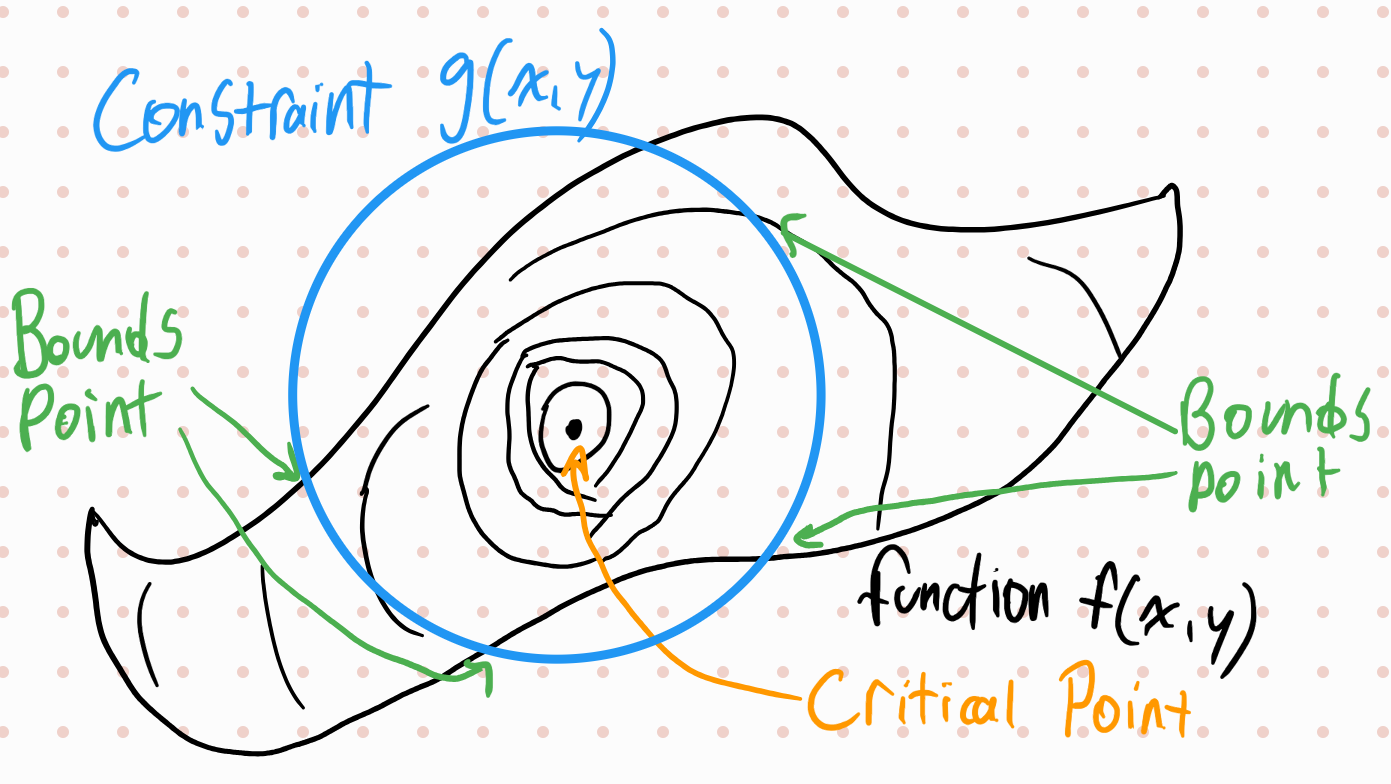
\includegraphics[width=0.5\linewidth]{lagrange.png}
	\end{figure}

	\begin{mdframed}[]
		\textbf{Ex. } Find the maximum and minimums of $f(x,y) = x^2+y^2 +4x-4y$ on $x^2+y^2\le 9$.
		
		We start by finding the crit points by setting $f_x=f_y=0$.
		\begin{align*}
			2x+4=0 \implies x=-2 \qquad 2y-4 = 0 \implies y=2
		\end{align*}
		We have a point $(0,0)$.
		
		Now we need to use lagrange multiplyers. 
		\begin{align*}
			& 2x+4 = \lambda 2x \implies \lambda = \frac{2x+4}{2x} \qquad 2y-4 = \lambda 2y \implies \lambda = \frac{2y-4}{2y}\\
			& \frac{2y-4}{2y} = \frac{2x+4}{2x} \qquad \implies \qquad x=-y
		\end{align*}
		Now subbing this into the constraint, we get:
		\begin{align*}
			y^2 + y^2 = 9 \implies y=\frac{\pm 3}{\sqrt{2}}
		\end{align*}
		Since we know that $x=-y$, we have 2 more points of: $\left(\frac{3}{\sqrt{2}},\frac{-3}{\sqrt{2}}\right)$, $\left(\frac{-3}{\sqrt{2}},\frac{3}{\sqrt{2}}\right)$
		
		Then we can take those 3 points, check which one is the min/max, and we are done.
	\end{mdframed}

	We can also do lagrange multipliers using 2 constraints.
	\begin{align*}
		\nabla f = \lambda \nabla g + \mu \nabla h
	\end{align*}
	
	\section{Double Integrals in Rectangular Regions [L6, L7]}
	It is easy to integrate a rectangular region of $R = [a,b] \times [c,d]$ by doing:
	\begin{align*}
		V = \int^b_a \int^d_c f(x,y) dxdy
	\end{align*}
	We can also change the order of integration and do the dx first or dy first (ensure to also change the bounds if changing the order).
	
	We just solve the first integral, and then solve the second integral using the result from the first integral.
	\begin{mdframed}[]
		\textbf{Ex. } Find the volume of $\int_R \int x-3y^2 dA$ on $R=[0,2]\times [1,2]$.
		
		We just add the x bounds (0,2) and y bounds (1,2) to the integral and solve to get:
		\begin{align*}
			\int^2_0 \int_1^2 x-3y^2 dydx = \int_0^2 x-7 dy = -12
		\end{align*}
	\end{mdframed}
	
	\section{Double Integrals in General Regions [L8]}
	This is very similar to double integrals in rectangular regions except that $dxdy \ne dydx$.
	
	To determine whether to do dxdy or dydx, we check if it is a type 1 or type 2 integral.
	
	For a type 1 integral, (functions are horizontal) we do:
	\begin{figure}[H]
		\centering
		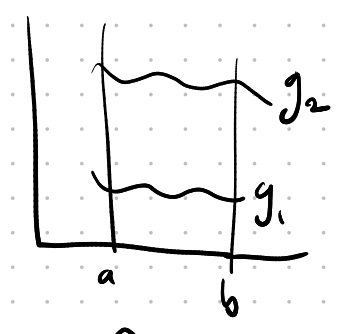
\includegraphics[width=0.3\linewidth]{type1.png}
	\end{figure}
	\begin{align*}
		\int_a^b \int^{g_2}_{g_1} f(x,y) dydx
	\end{align*}

	For a type 2 integral (functions are vertical) , we do:
	\begin{figure}[H]
		\centering
		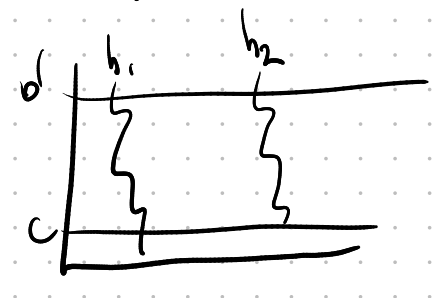
\includegraphics[width=0.3\linewidth]{type2.png}
	\end{figure}
	\begin{align*}
		\int_a^b \int_{h_1}^{h_2} f(x,y) dxdy
	\end{align*}
	
	\section{Polar Coordinates [L8, L9, L10]}
	When we are working with polar coordinates, rather than using the x and y, we use r and $\theta$ where r is the radius, and $\theta$ is the angle from the positive x axis. 
	
	To convert from cartesian to polar, we use:
	\begin{align*}
		x = r\cos(\theta) \qquad y = r\sin(\theta)\\
		\int_R \int f(x,y) dA = \int^{\beta} _{\alpha} \int^b_a f(r\cos\theta,r\sin\theta)\cdot r\cdot drd\theta
	\end{align*}
	
	\begin{mdframed}[]
		\textbf{Ex. } Find the shaded area:
		\begin{figure}[H]
			\centering
			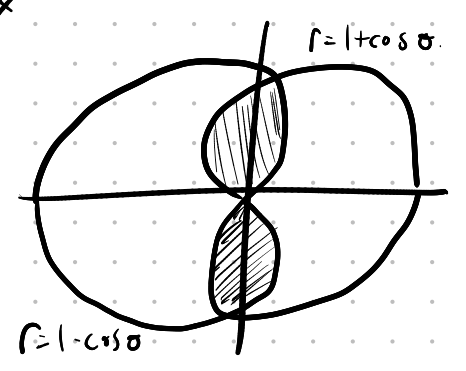
\includegraphics[width=0.4\linewidth]{figure.png}
		\end{figure}
	
		We are not sure how to do this using cartesian coordinates. It looks simple with polar though.
		
		We see that the radius at any point on the top half is just 0 to the function $1+\cos\theta$. The angle goes through the whole $2\pi$ but we will just do half of that, and then double the integral. It goes from $-\pi/2$ to $\pi/2$.
		\begin{align*}
			2\cdot \int^{\frac{\pi}{2}}_\frac{-\pi}{2} \int_0^{1+\cos\theta} r\cdot drd\theta = SOLVE
		\end{align*}
	\end{mdframed}

	
	\section{Applications of Double Integrals [L11]}
	
	We analyse 4 applications in this course.
	
	\subsection{Finding Mass from Density}
	Generally we are given a density function $\rho (x,y)$ and we need to find the mass of a domain $D$ from that, we use the following integral:
	\begin{align*}
		m = \iint\limits_D \rho(x,y) dA
	\end{align*}
	
	\subsection{Finding center of mass}
	To find this, we need to know the moment equations using the density $\rho$ on the domain $D$.
	\begin{align*}
		M_x = \iint\limits_D y\rho(x,y) da \qquad M_y = \iint\limits_D x\rho(x,y)
	\end{align*}
	Then we can get the center of mass:
	\begin{align*}
		\overline{x} = \frac{M_y}{m} \qquad \overline{y} = \frac{M_x}{m}
	\end{align*}
	
	\subsection{Inertia}
	This is very similar to the center of mass:
	\begin{align*}
		I_x = \iint\limits_D y^2 \rho(x,y) dA \qquad I_y = \iint\limits_D x^2 \rho(x,y)dA \qquad I = \iint\limits_D \left(x^2 + y^2 \right) \rho(x,y) dA
	\end{align*}
	
	
	\section{Surface Area [L12]}
	The surface area of a function $f$ on a domain $D$ 	can be calculated as:
	\begin{align*}
		A(s) =  \iint\limits_D \sqrt{\left(\frac{\partial f}{\partial x} \right)^2 + \left(\frac{\partial f}{\partial y}\right)^2 + 1} dA
	\end{align*}

	\section{Change of Variables [L13]}
	Whenever we perform a transformation on a function (such as rectangular coordinates to polar coordinates), we need to multiply by a factor known as the \textbf{Jacobian}
	
	Recall that with the polar coordinates, we had to always multiply by a factor of $r$, this is because of the Jacobian.
	\begin{align*}
		J = \frac{\partial (x,y) }{\partial (u,v)} = \left|\begin{array}{cc} \frac{\partial x}{\partial u} & \frac{\partial x}{\partial v} \\ \frac{\partial y}{\partial u} & \frac{\partial y}{\partial v} \end{array}\right|
	\end{align*}
	
	\section{Triple Integrals [L14]}
	We have 3 types of triple integrals:
	
	\begin{figure}[H]
		\centering
		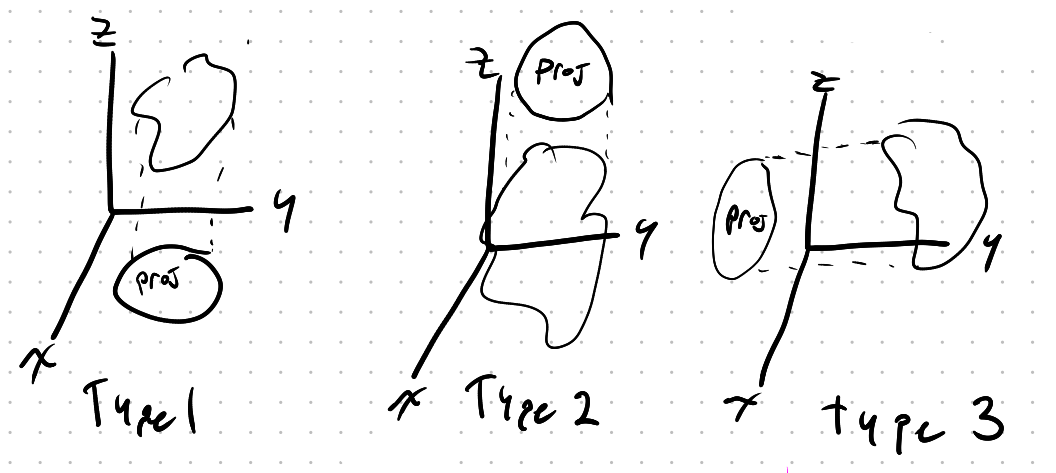
\includegraphics[width=0.7\linewidth]{screenshot001}
	\end{figure}
	
	\section{Triple Integrals in Cylindrical Coordinates [L15, L16]}
	In cylindrical coordinates, we convert $(x,y,z) \to (r,\theta, z)$ where:
	\begin{align*}
		x = r\cdot \cos(\theta) \qquad y = r\cdot \sin(\theta) \qquad z = z
	\end{align*}
	Then we have the jacobian of $J=r$.
	
	We can use logic to reason that $r =\sqrt{x^2+y^2}$, and $\theta = \arctan\left(\frac{x}{y}\right)$.
	
	\section{Triple Integrals in Sperical Coordinates [L15, L16]}
	In spherical coordinates we convert $(x,y,z) \to (\rho, \theta, \phi)$ where:
	\begin{align*}
		x = \rho \cos(\theta) \sin(\phi) \qquad y = \rho \sin(\theta) \sin(\phi) \qquad z = \rho \cos(\phi)
	\end{align*}
	We have the jacobian of: $J = \rho^2 \sin(\phi)$
	
	Then we can reason that $x^2 + y^2 + z^2 = \rho ^2$.
	
	
	
\end{document}